\documentclass{standalone}
\usepackage[dvipsnames,svgnames,x11names]{xcolor}
\usepackage{tikz}
\usepackage{pgfplots}
\pgfplotsset{compat = 1.12}
\usepackage{../thesismath}
\begin{document}
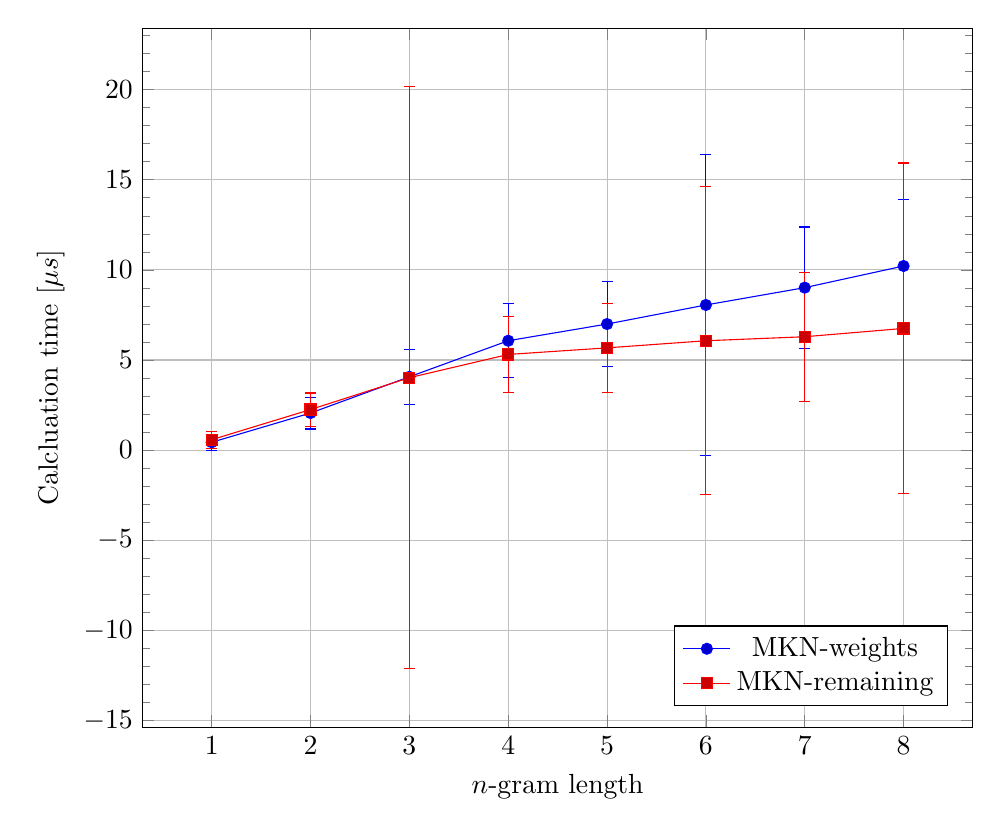
\begin{tikzpicture}[baseline]

\begin{axis}[
  xlabel = {$n$-gram length},
  xtick = {1, ..., 8},
  ylabel = {Calcluation time [$\mu s$]},
  minor y tick num = 4,
  grid = major,
  legend entries = {{MKN-weights}, {MKN-remaining}},
  legend pos = south east,
  width = \textwidth,
]

% MKN-weights
\addplot+[
  error bars/.cd,
  y dir = both,
  y explicit,
] table [y error = us_error] {
  n  us      us_error
  1   0.434   0.444
  2   2.056   0.886
  3   4.065   1.513
  4   6.067   2.045
  5   6.993   2.343
  6   8.051   8.331
  7   9.013   3.367
  8  10.213   3.707
};

% MKN-remaining
\addplot+[
  error bars/.cd,
  y dir = both,
  y explicit,
] table [y error = us_error] {
  n  us      us_error
  1   0.577   0.466
  2   2.249   0.918
  3   4.016  16.159
  4   5.306   2.089
  5   5.672   2.485
  6   6.066   8.538
  7   6.289   3.581
  8   6.750   9.179
};

\end{axis}

\end{tikzpicture}
\end{document}
